\documentclass{article}
\usepackage[utf8]{inputenc}
\usepackage{url}

\title{Assignment 3 EECS 410}
\author{Madison Hillyard }
\date{October 26, 2020}

\usepackage{natbib}
\usepackage{graphicx}
\usepackage{subfig}
\usepackage{float}

\begin{document}

\maketitle

\section{Introduction}
This assignment covered the creation of a health self-management application. The main function of this application is to allow the user to track their Hashimoto's Disease medicine Synthroid. To do this the application, called Hashimoto's Tracker, uses not only the user's movement but also their calendar for reminders. Using this the application then tracks the number of days the patient takes their pill at the correct time. This Application uses both Android's Embedded Calendar \citep{AndroidCalendar} and Location \citep{SmartLocation} services. The physical location of the user is show using the a combination of Google Maps API\citep{GoogleMaps} and a library called SmartLocation\citep{SmartLocation}.

To facilitate the data persistence through out the use of the application the application uses the Room Library to handle all SqlLite operations. This enables robust data-typing as well as query verification at compile time to handle query errors before the application reaches the user. The databases directory provided with this document shows an example of the data held in the database. This directory contains three files: tracking\_database.db, tracking\_database.db-wal and tracking\_database.db-shm. To view or use this database all three files must be present in your working directory.

This application allows the user to track their medication intake over time and promotes more timely and consistent use. Users are able to visualize their consistency and are reminded when they are late.  This can be used to better maintain user's level of hormone and improve their overall physical health.

\section{Related Work}
Hashimoto's Disease, as well as Hypothyroidism are incurable diseases that require timely and consistent medical intervention. Patients that suffer from hypothyroidism must consume their Synthroid at regular intervals to maintain the correct level of hormone throughout their body. Synthroid, or it's generic brand counterpart Levothyroxine, should be taken on an empty stomach, at the same time everyday and with no food. 

\begin{figure}[H]
\centering
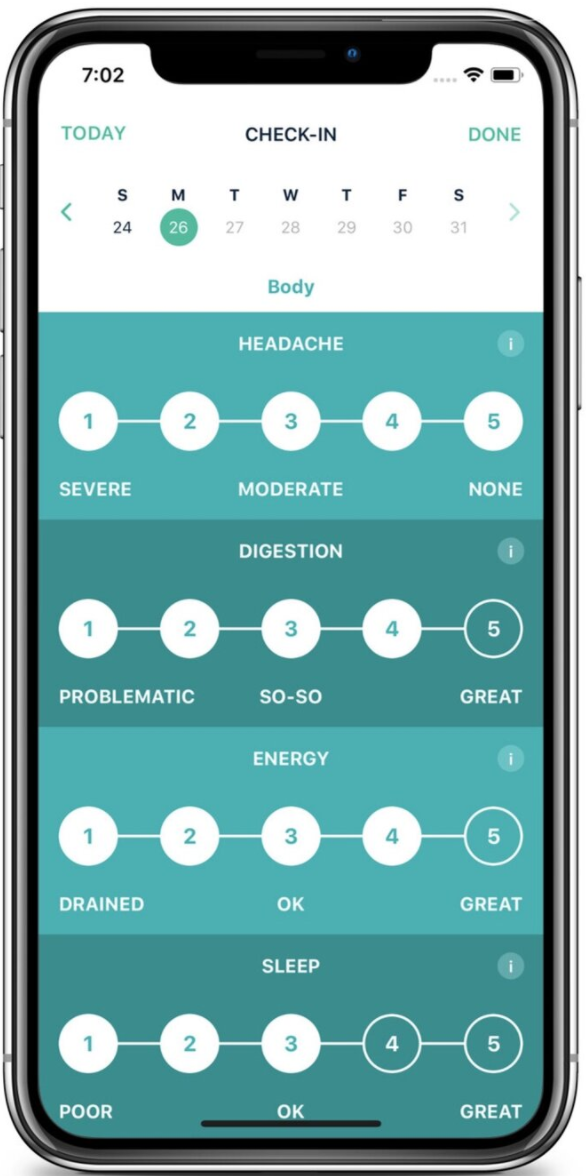
\includegraphics[scale= .2]{img/boostThyroid.PNG}
\caption{The Boost Thyroid App}
\label{fig:boost} 
\end{figure}

The application that I found that helps people with Hashimoto's is Boost Thyroid. Boost is a general thyroid/health tracker application made for iOS. It allows you to track and visualize your symptoms and lab results. The application identifies the most common symptoms that patients with diseased thyroids experience and allows you to track those and more over time. The lab test tracker allows the user to track specific lab results such as TSH anti-TPO and anti-TG.

Not only is the tracking function helpful to a patients understanding of their disease the app also helps patients understand their diagnosis.  The application gives the user general knowledge about the most common tests and symptoms that they will see over time with their diagnosis. Most patients struggling with hypothyroidism are required to get lab tests done multiple times a year and will need their medication levels changed due to their body changing over time. 

Boost also allows users to track lab results in relation to their fertility. For women, fertility can be greatly affected by hypothyroidism. The intersectionality of Boost is a great example of further improvements. \citep{boost}

\begin{figure}[H]
  \centering
  \subfloat[Thyroid Tracker Menu.]{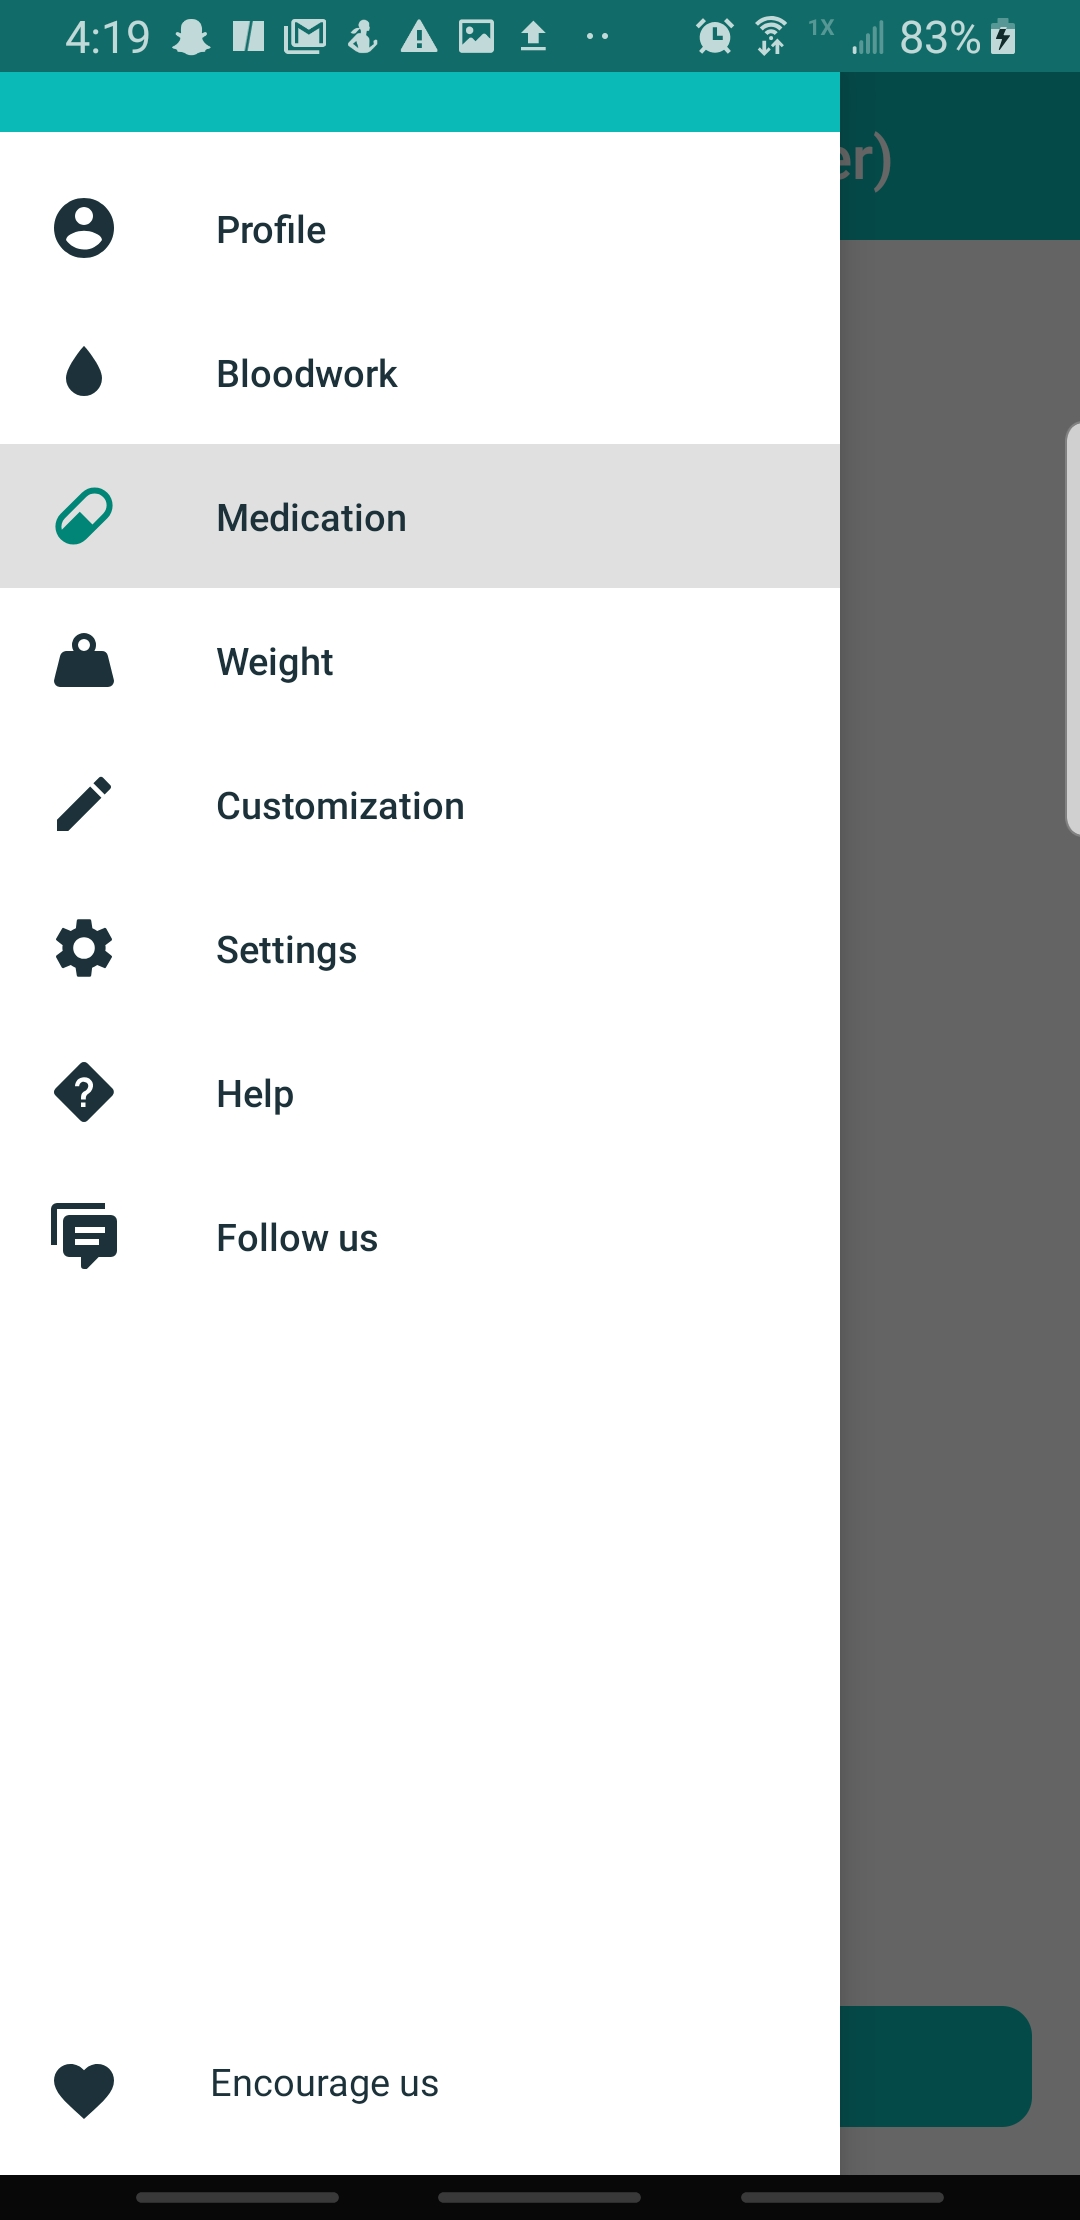
\includegraphics[scale=.07]{img/thy_menu.jpg}\label{fig:nike_run1}}
  \hfill
  \subfloat[Thyroid Tracker Medication Screen.]{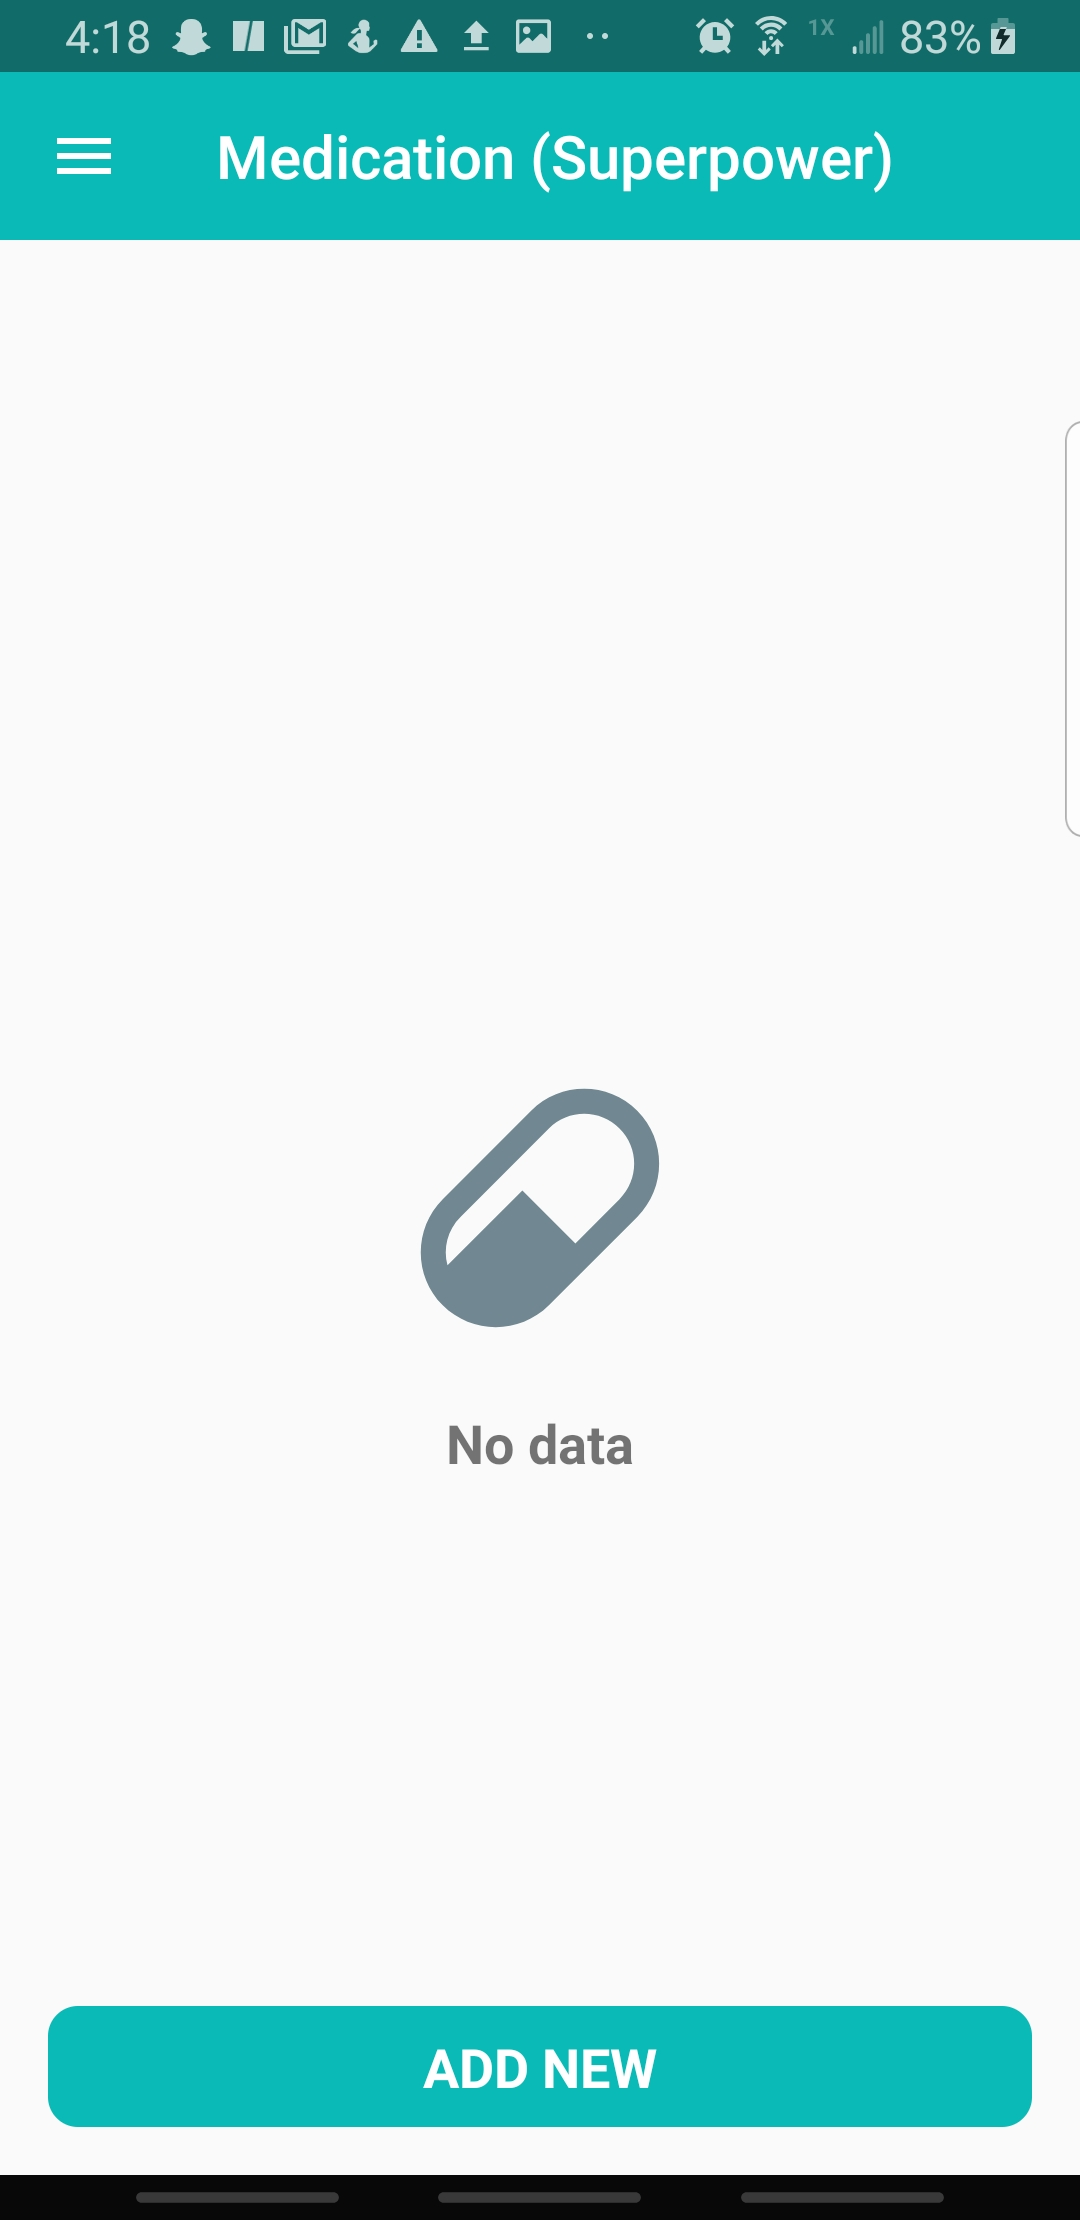
\includegraphics[scale=.07]{img/thy_med.jpg}\label{fig:nike_run2}}
  \caption{Two examples of the Thyroid Tracker user interface }
\end{figure}

Another good example of an Android application for thyroid tracking is Thyroid Tracking. This application combines the functionality of Boost with metrics to track weight and reminder settings. The addition of weight is important. One of the main symptoms of Hashimoto's is inability to gain or lose weight. This application could easily be used by patients in between appointments to track their symptoms.\citep{ThyroidTracker}

Further places of intersectionality between hypothyroidism and other health concerns could be in gut symptom and food tracking. Patients with Hashimoto's have a very high chance of developing Celiac Disease or of being lactose intolerant. In the future applications that allows for users to track symptoms across diseases will make a huge impact.



\section{System Overview}
The System has four main states, three main user inputs, and a BroadcastReciever that creates a notification pointing back to the main activity. The user inputs do not include the closing and pausing of app. The pausing of the application is the same as pausing will not stop the location services. The closing of the application will not erase the backend database, all data will persist.

\begin{figure}[H]
\centering
\includegraphics[scale=.55]{img/Assignment 3.pdf}
\caption{The System}
\label{fig:system}
\end{figure}

There are three main flows of user interface information, a Broadcast Receiver flow and a Database updater flow. 

\subsection{Database Flow}
On creation of the main Activity, if the database is empty a tracker entity will be added. This tracker will be updated by the application using a callback in the main activity. The updating process allows the application to treat the database as the point of truth in the system.

\subsection{Tracking Flow}
On creation of the main activity the application queries the latest tracking numbers for the UI. When either of the track or miss buttons are pressed the database is updated and the callback from the database flow updates the UI.

\subsection{GeoFence Flow}
On creation of the main activity the application requests location permissions. When you navigate to the GeoFence Page the Google Maps MapView is initialized and your location is used to center the map. The GeoFence Radius Slider controls the radius parameter. When the Set GeoFence Button is pressed the main Activity creates a new GeoFence and starts it. This button also updates the database and the callback from the database flow updates the UI.

\subsection{Reminder Flow}
After navigating the Set Reminder Page and pressing the set reminder button the application updates the database and then sends a CalendarContract Object to the calendar of the user's choosing. The database then updates the UI using the callback in the main activity.

\begin{figure}[H]
\centering
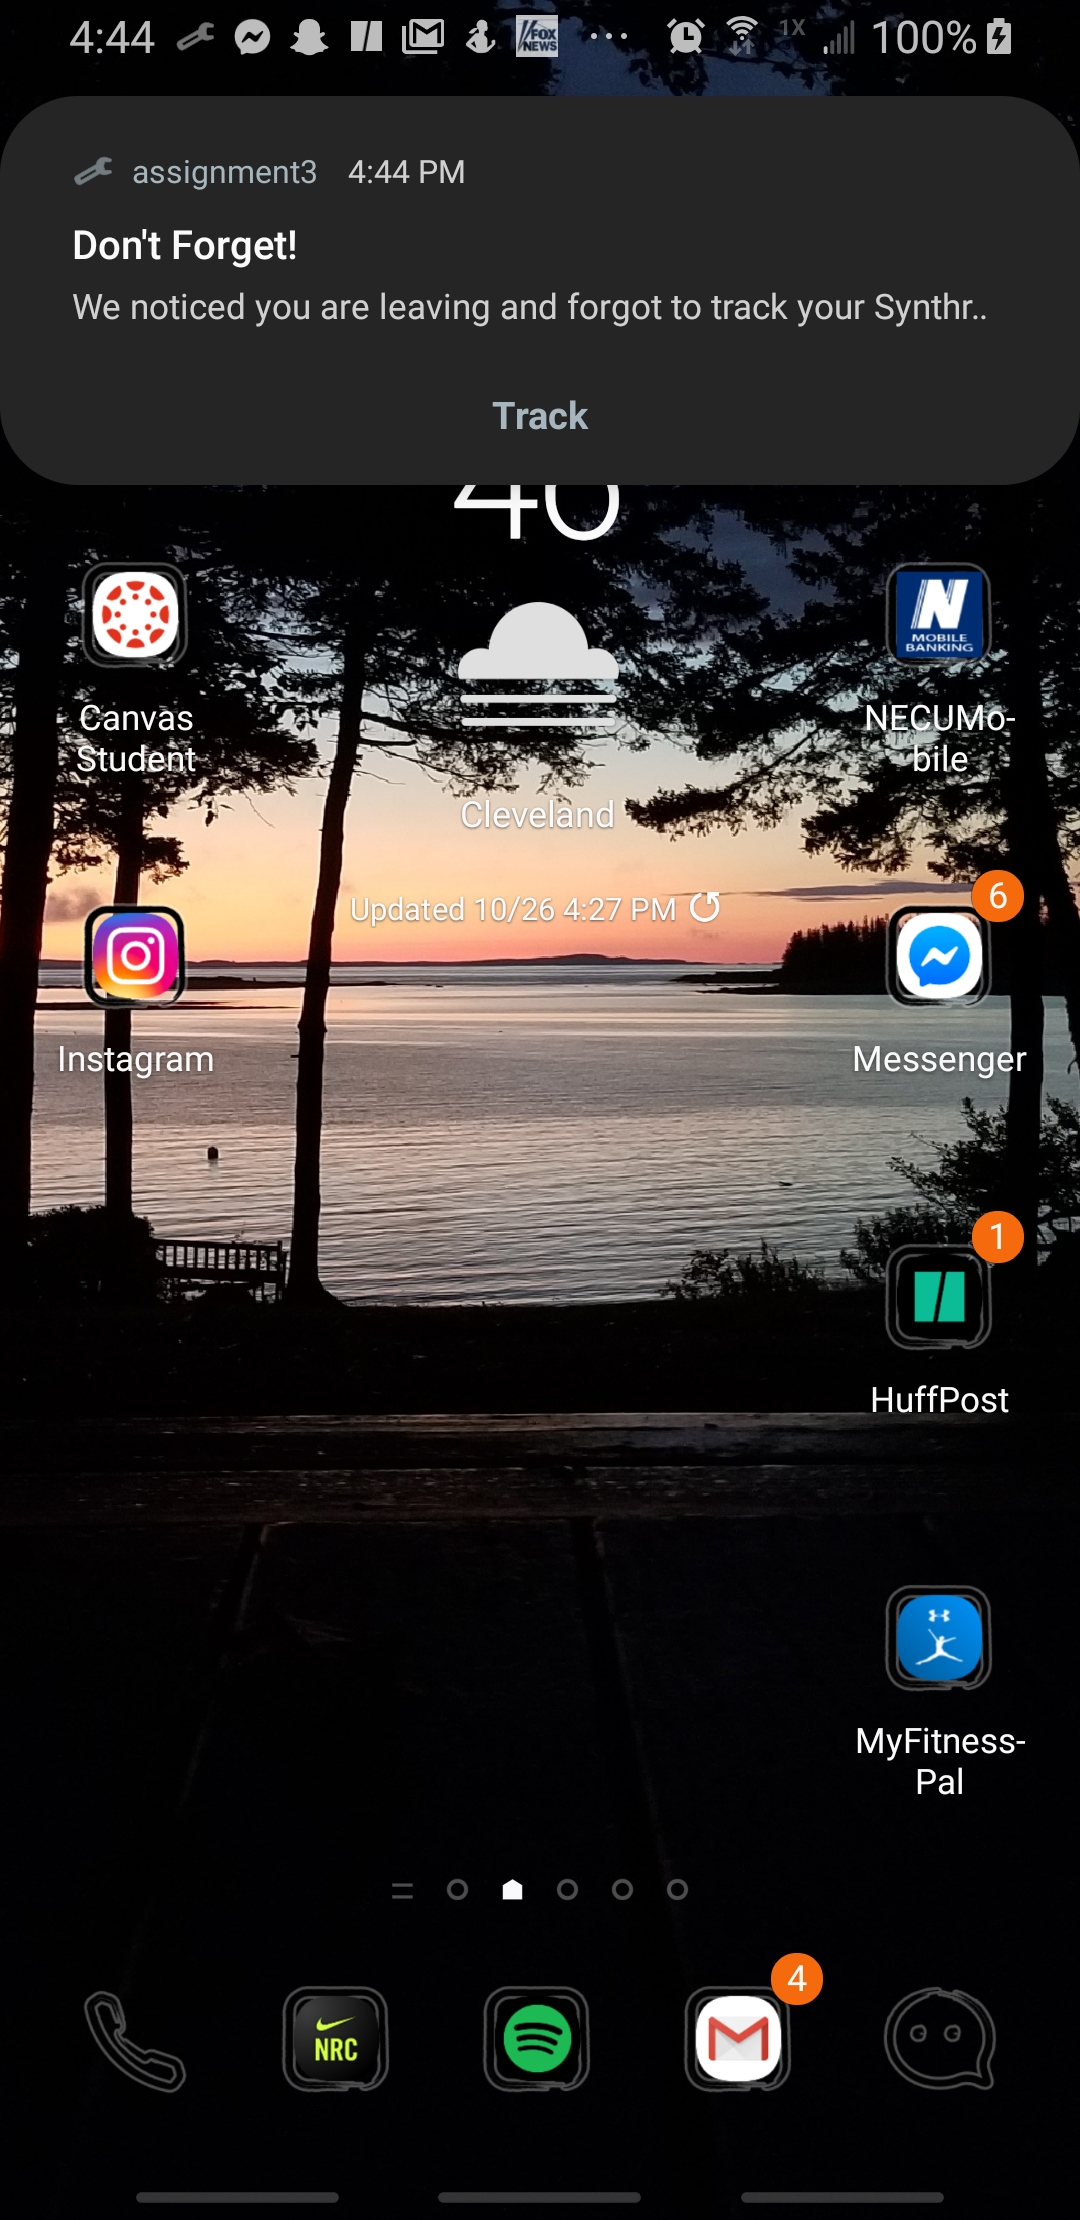
\includegraphics[scale= .1]{img/notification.jpg}
\caption{Example of a Notification Form the Broadcast Receiver}
\label{fig:notification} 
\end{figure}

\subsection{Broadcast Receiver Flow}
On creation of the application, a broadcast receiver is created. Once a GeoFence Transition Exit is detected the Broadcast Receiver will issue a notification that reminds the user that they are leaving without tracking their medication.

Please note that Location and Notification permissions must be enabled.

\section{User Guide}
This application has five main parts: Tracker Home Page, Menu, Set Reminder Page, Set Location Page and Database Information.

\begin{figure}[H]
\centering
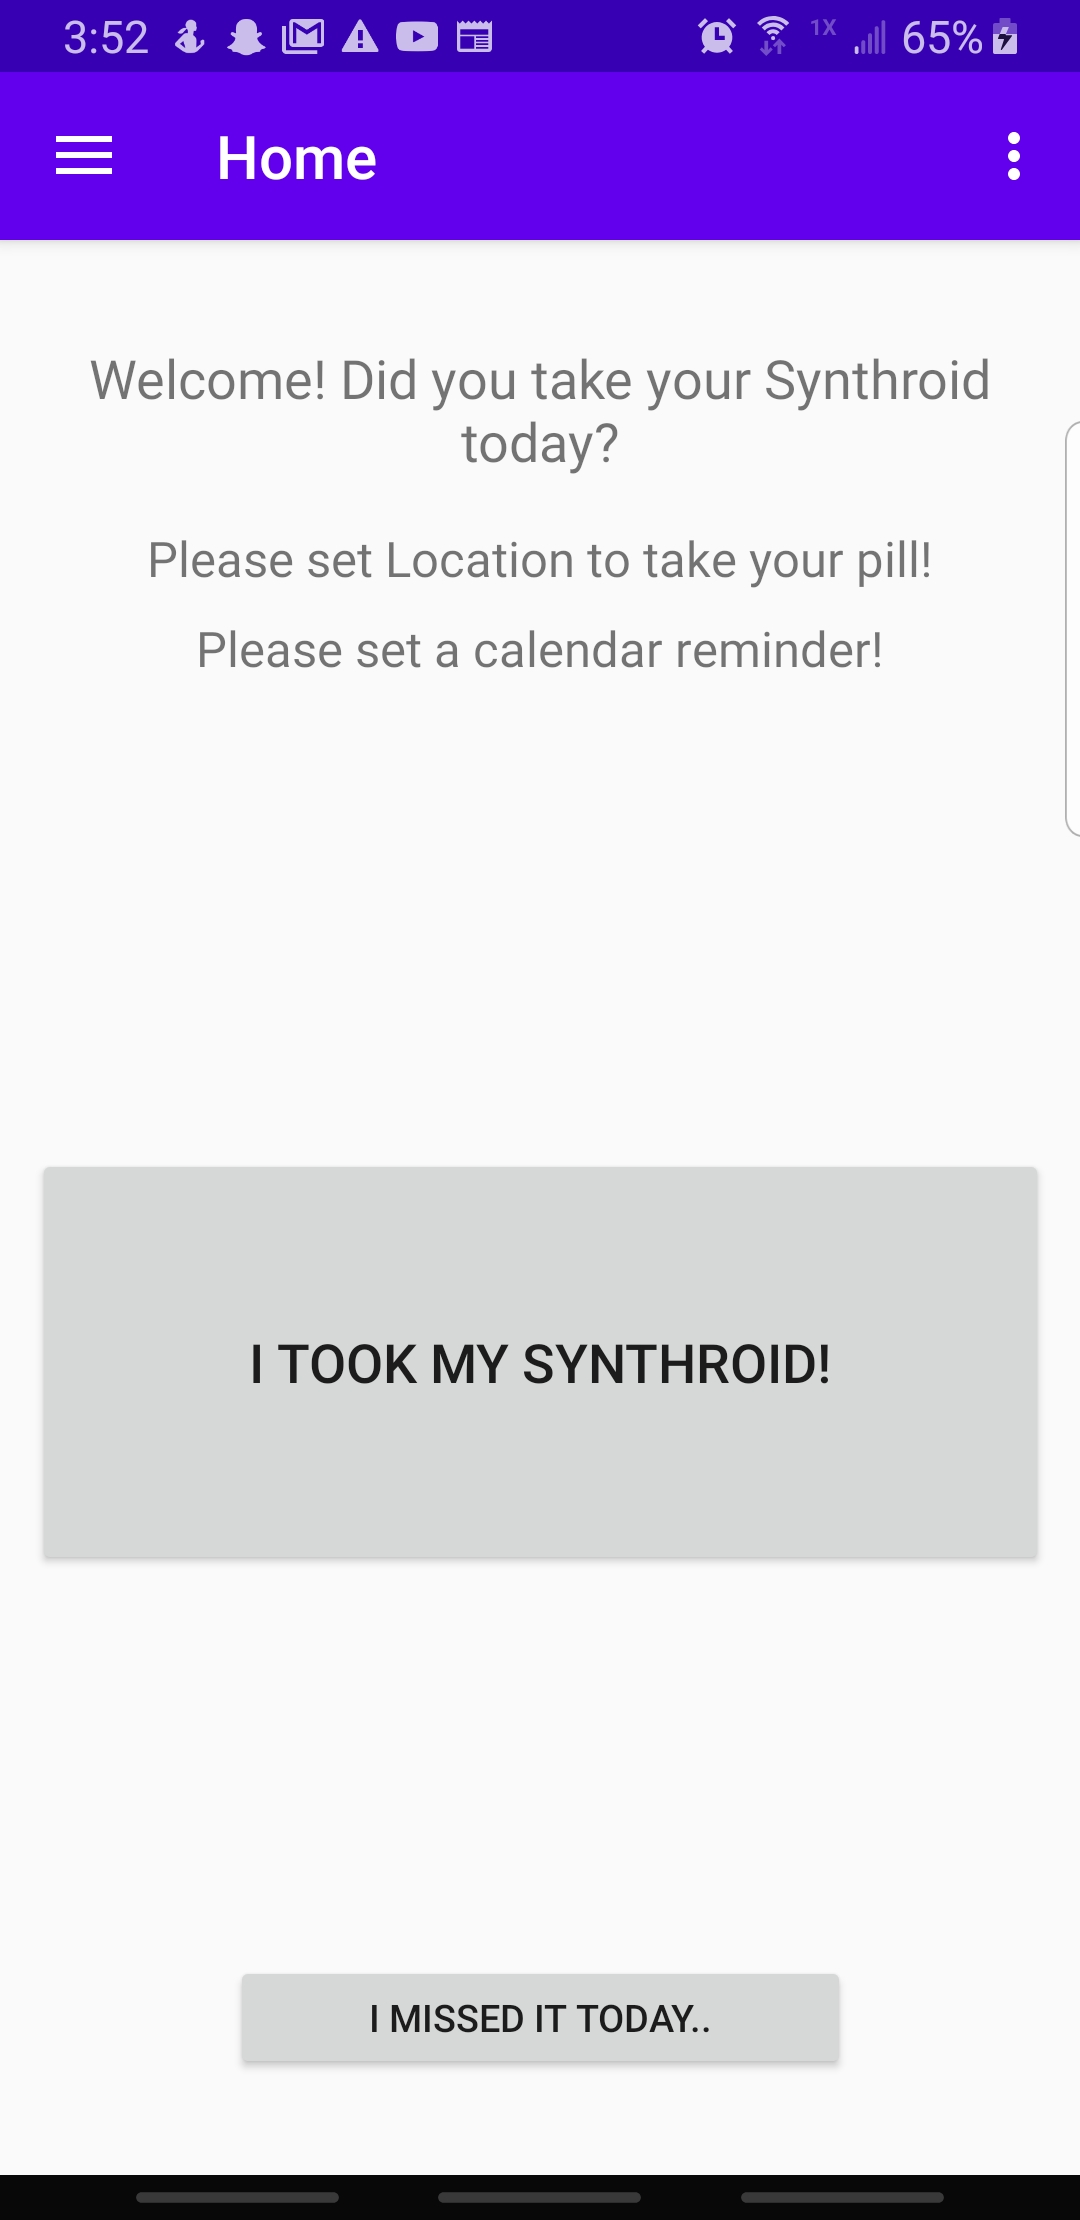
\includegraphics[scale= .1]{img/home.jpg}
\caption{Tracker Home Page}
\label{fig:home} 
\end{figure}

\subsection{Tracker Home}
This is the main page of the application. This page is where you track your medication usage.
\subsubsection{Information}
This is a few lines of test that tells you if you have set your location and reminders. If you see text telling you to go set your location or reminders navigate to those pages and set that information.
\subsubsection{Track Button}
This button when pressed tells the application that you took your medicine for the day.
\subsubsection{Miss Button}
This button when pressed tells the application that you missed your medication for the day.

\begin{figure}[H]
\centering
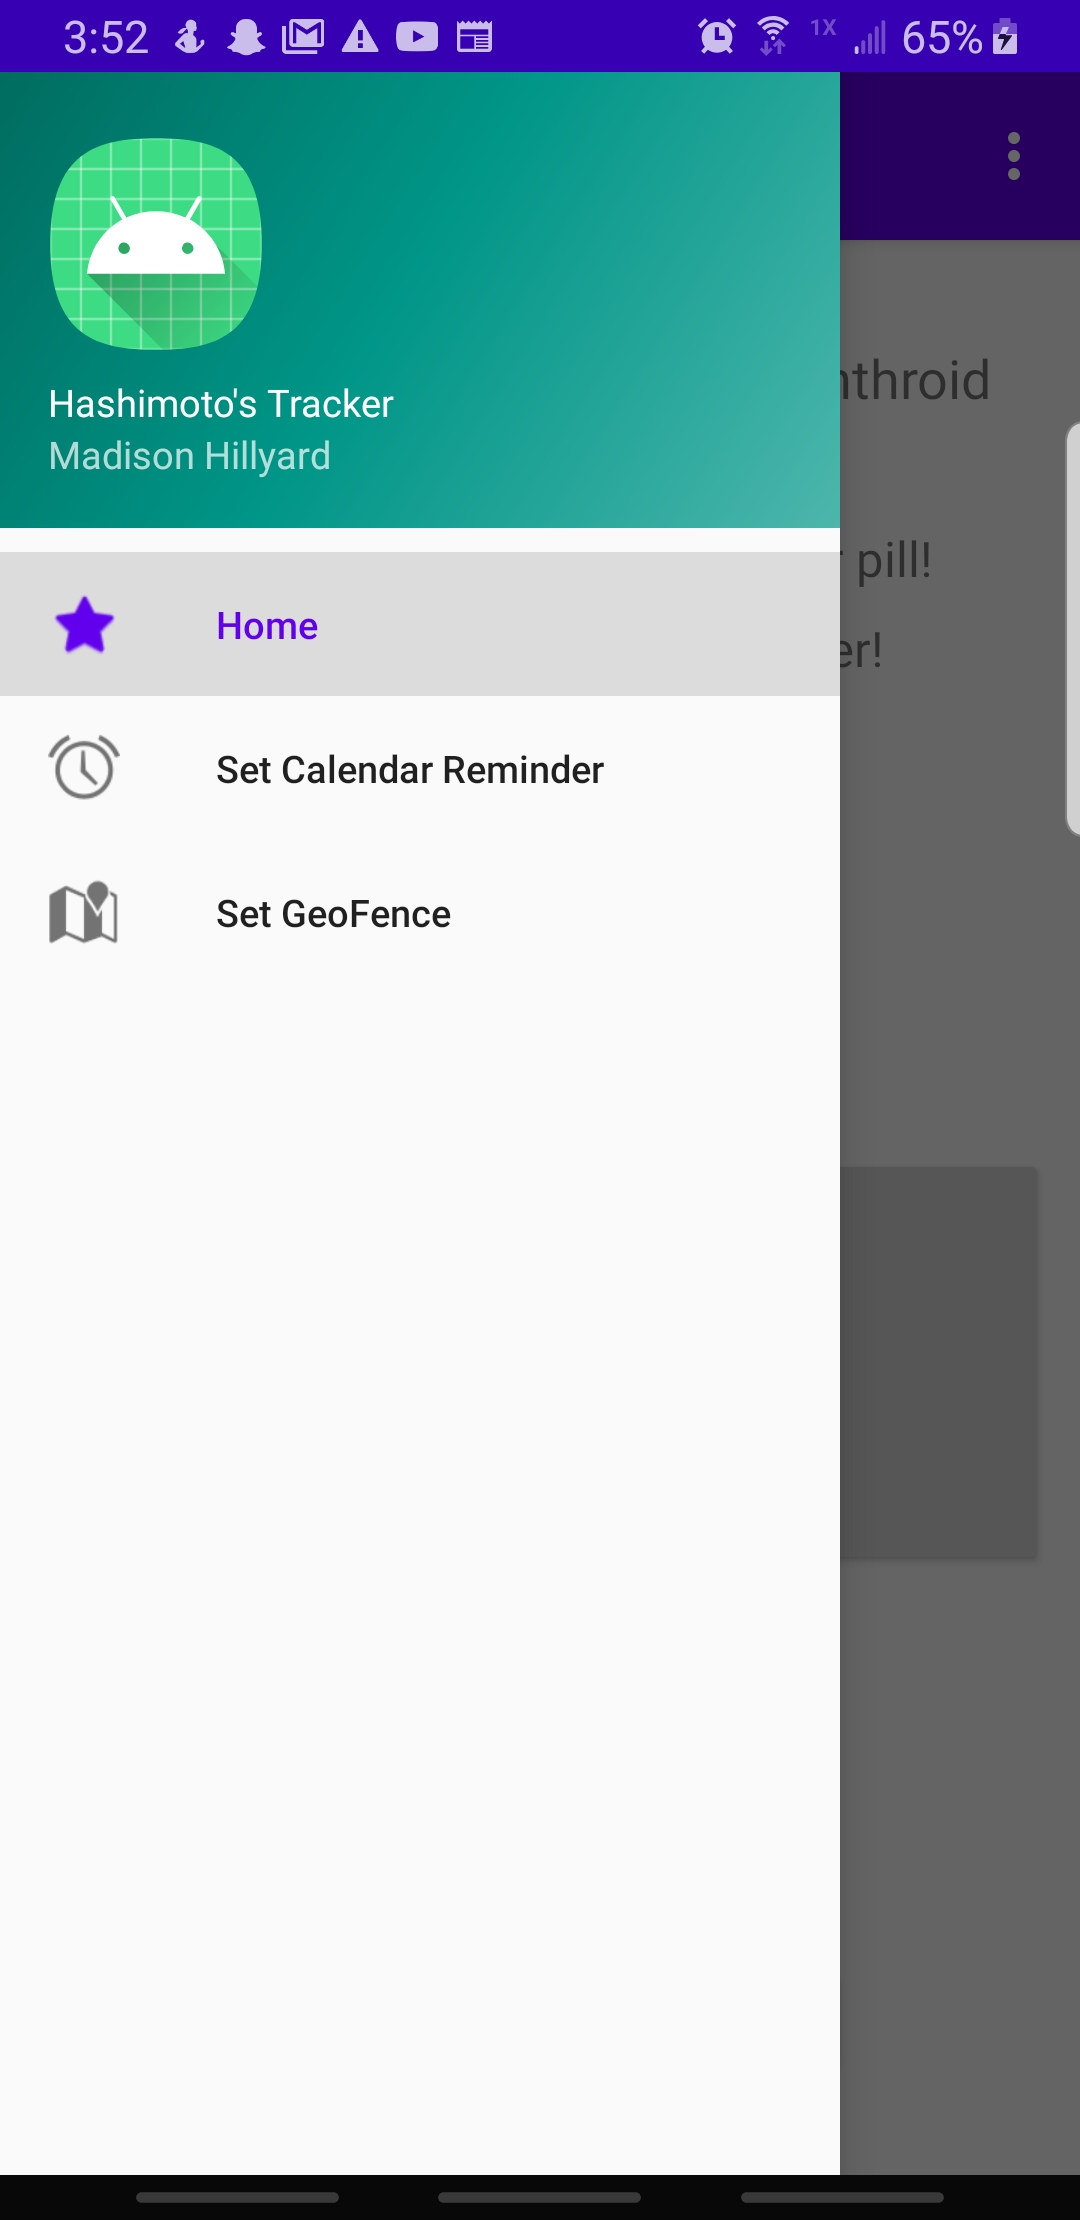
\includegraphics[scale= .1]{img/menu.jpg}
\caption{Menu Page}
\label{fig:menu} 
\end{figure}

\subsection{Menu}
The Menu is reached by pressing the menu button on the top left of the screen. The Menu consists of the main navigation of the application.
\subsubsection{Tracker Home Option}
This button will open the Tracker Home Page.
\subsubsection{Set Reminder Option}
This button will open the Set Reminder Page.
\subsubsection{Set Location Option}
This button will open the Set Location Page.

\begin{figure}[H]
\centering
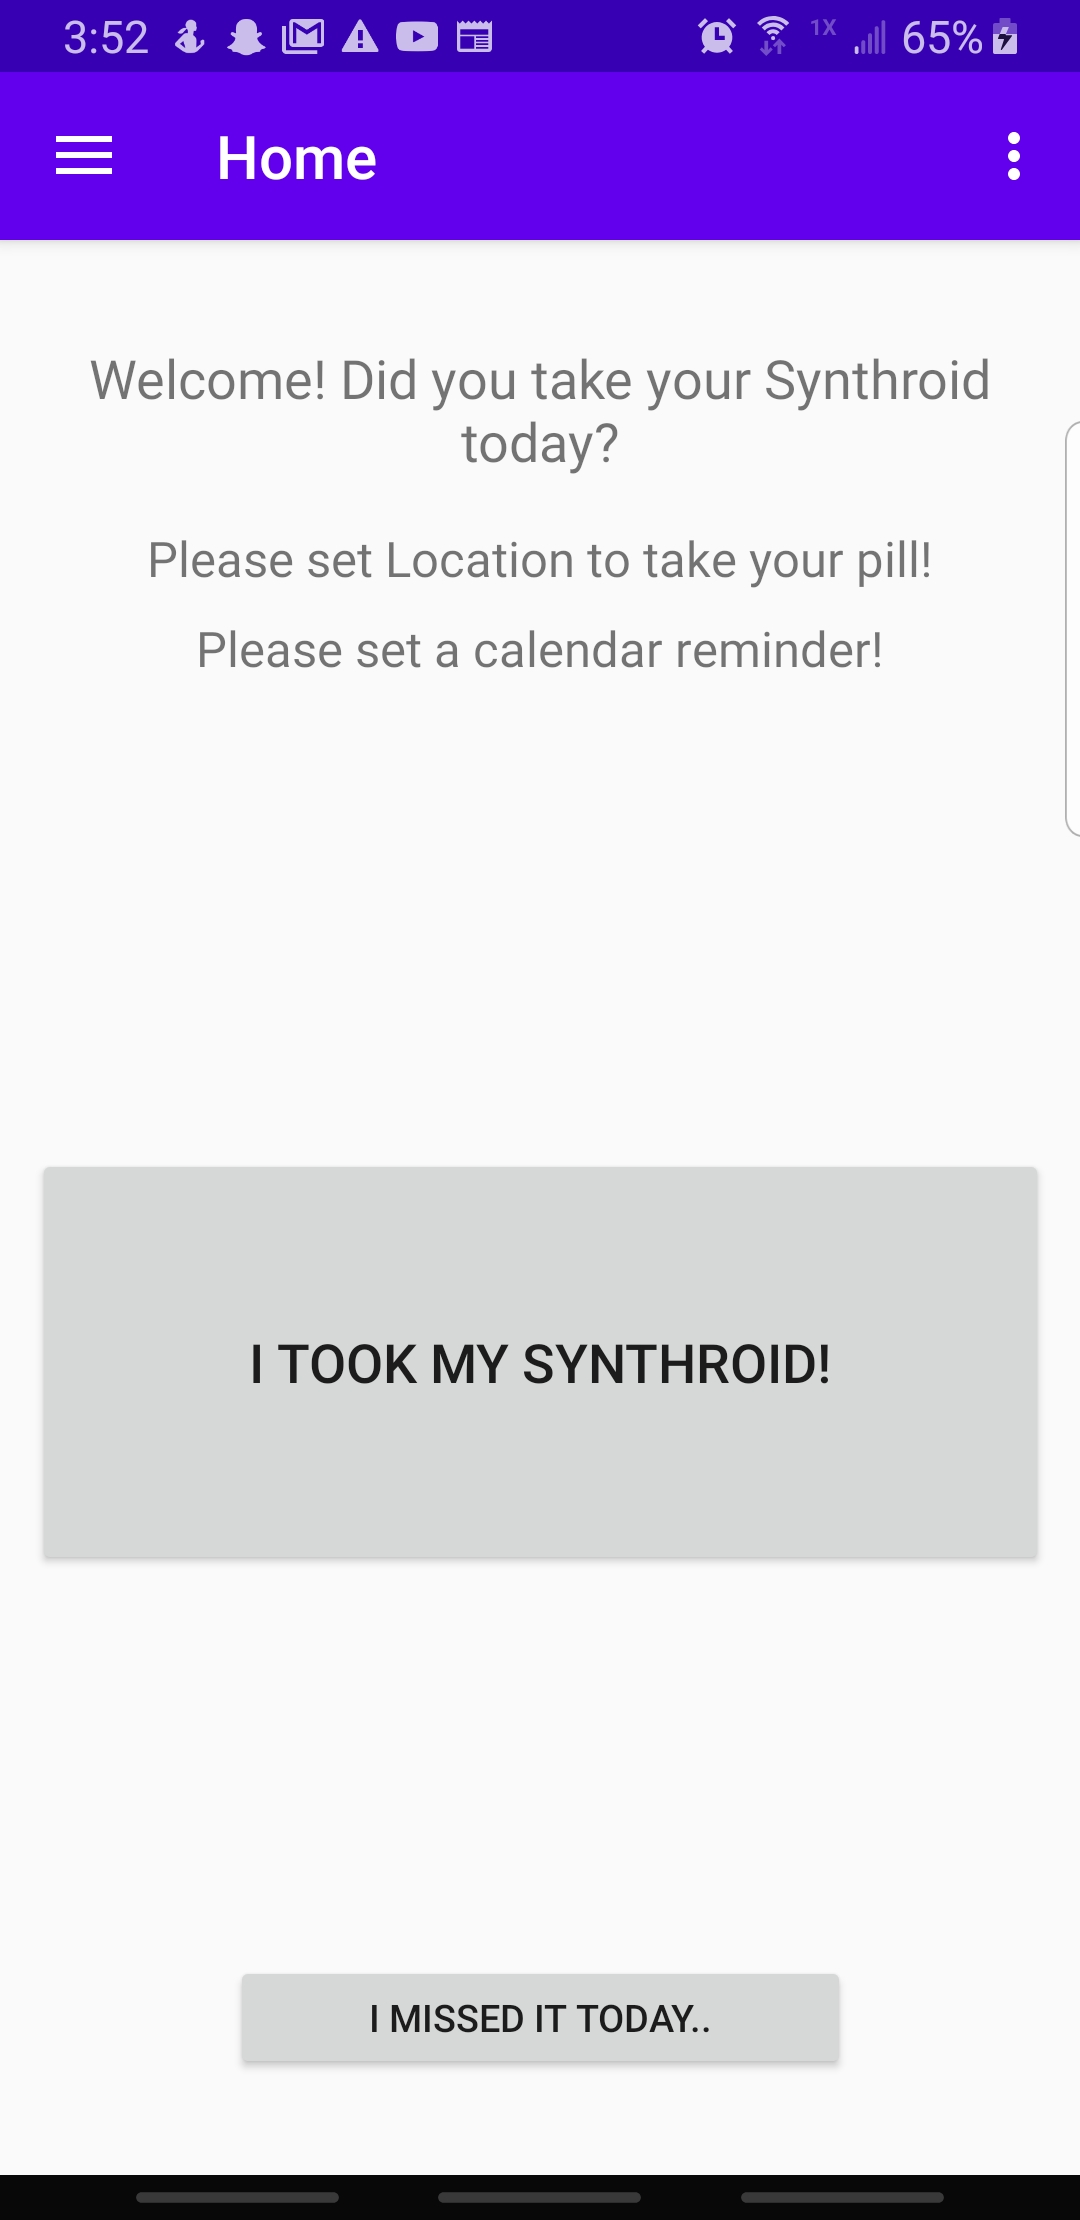
\includegraphics[scale= .1]{img/home.jpg}
\caption{The Set Reminder Page}
\label{fig:reminder} 
\end{figure}

\subsection{Set Reminder Page}
This page enables the user to set a  reminder at a specific time of day for their medication. 
\subsubsection{Set Time Button}
This button opens a Time Picker. When you have chosen the correct time click okay.
\subsubsection{Set Reminder Button}
This button starts opens up your preferred calendar application to set your reminder.

\begin{figure}[H]
\centering
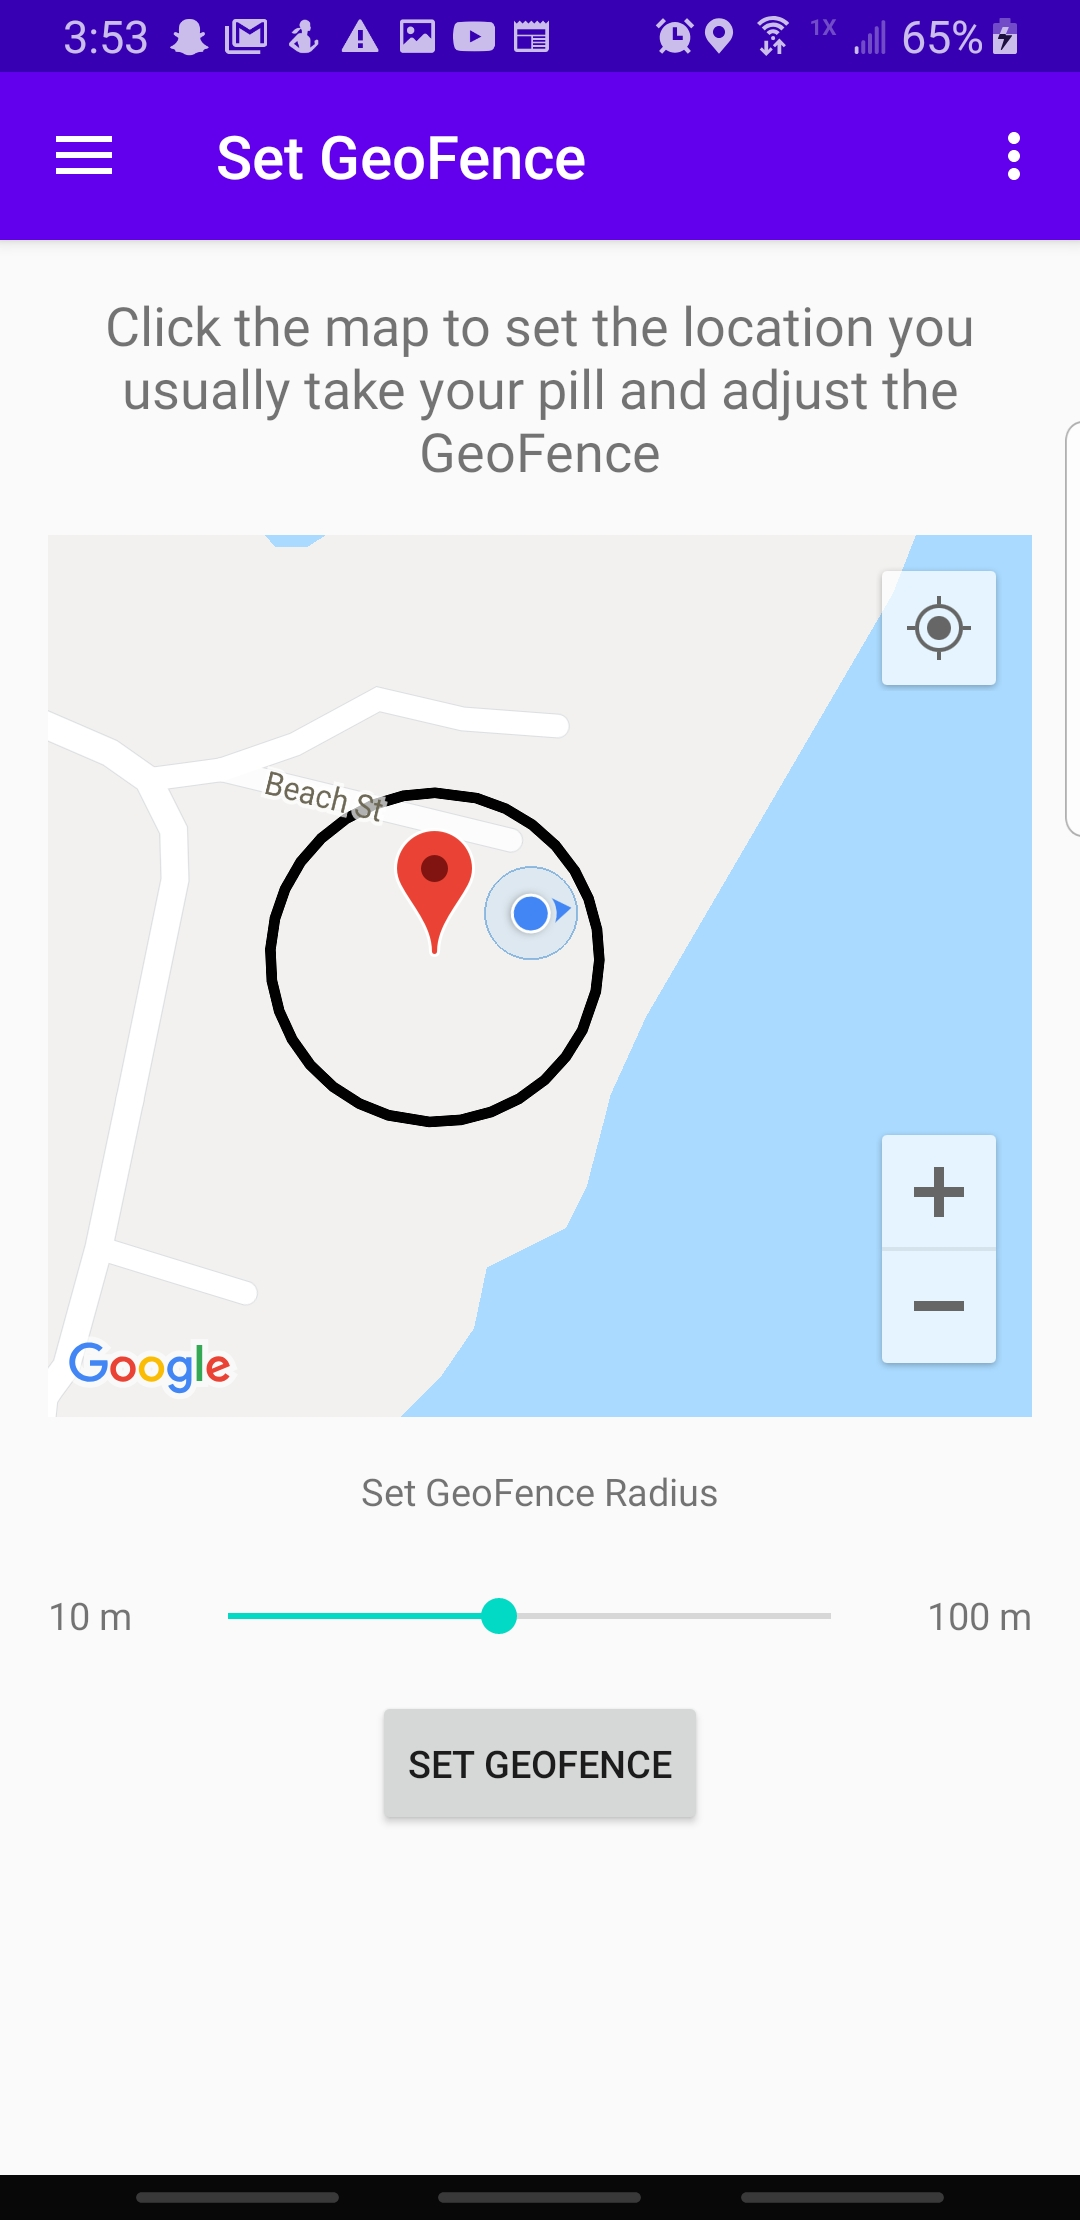
\includegraphics[scale= .1]{img/geofence.jpg}
\caption{The Set Location Page}
\label{fig:location} 
\end{figure}

\subsection{Set Location Page}
This page enables the user to set the location and geofence size for the place they are most commonly in the morning. Most users will pick home. The geofence can be moved when ever the user prefers and will persist. 
\subsubsection{Map}
The Map will open on you current location. Click on the map where you would like you geofence location to be. If you would like to set your current location as your geofence location either click your location or simply move onto the Geofence slider as your current location is pre-selected.
\subsubsection{Geofence Slider}
the geofence slider allows the user to set the radius of the geofence. The geofence slider ranges from 10m to 100m depending on the users preference. When you move to slider you will see the geofence circle extending from the location you chose.
\subsubsection{Set Location Button}
When you have chosen your location and geofence radius click the Set Location Button to register it with the application.

\begin{figure}[H]
\centering
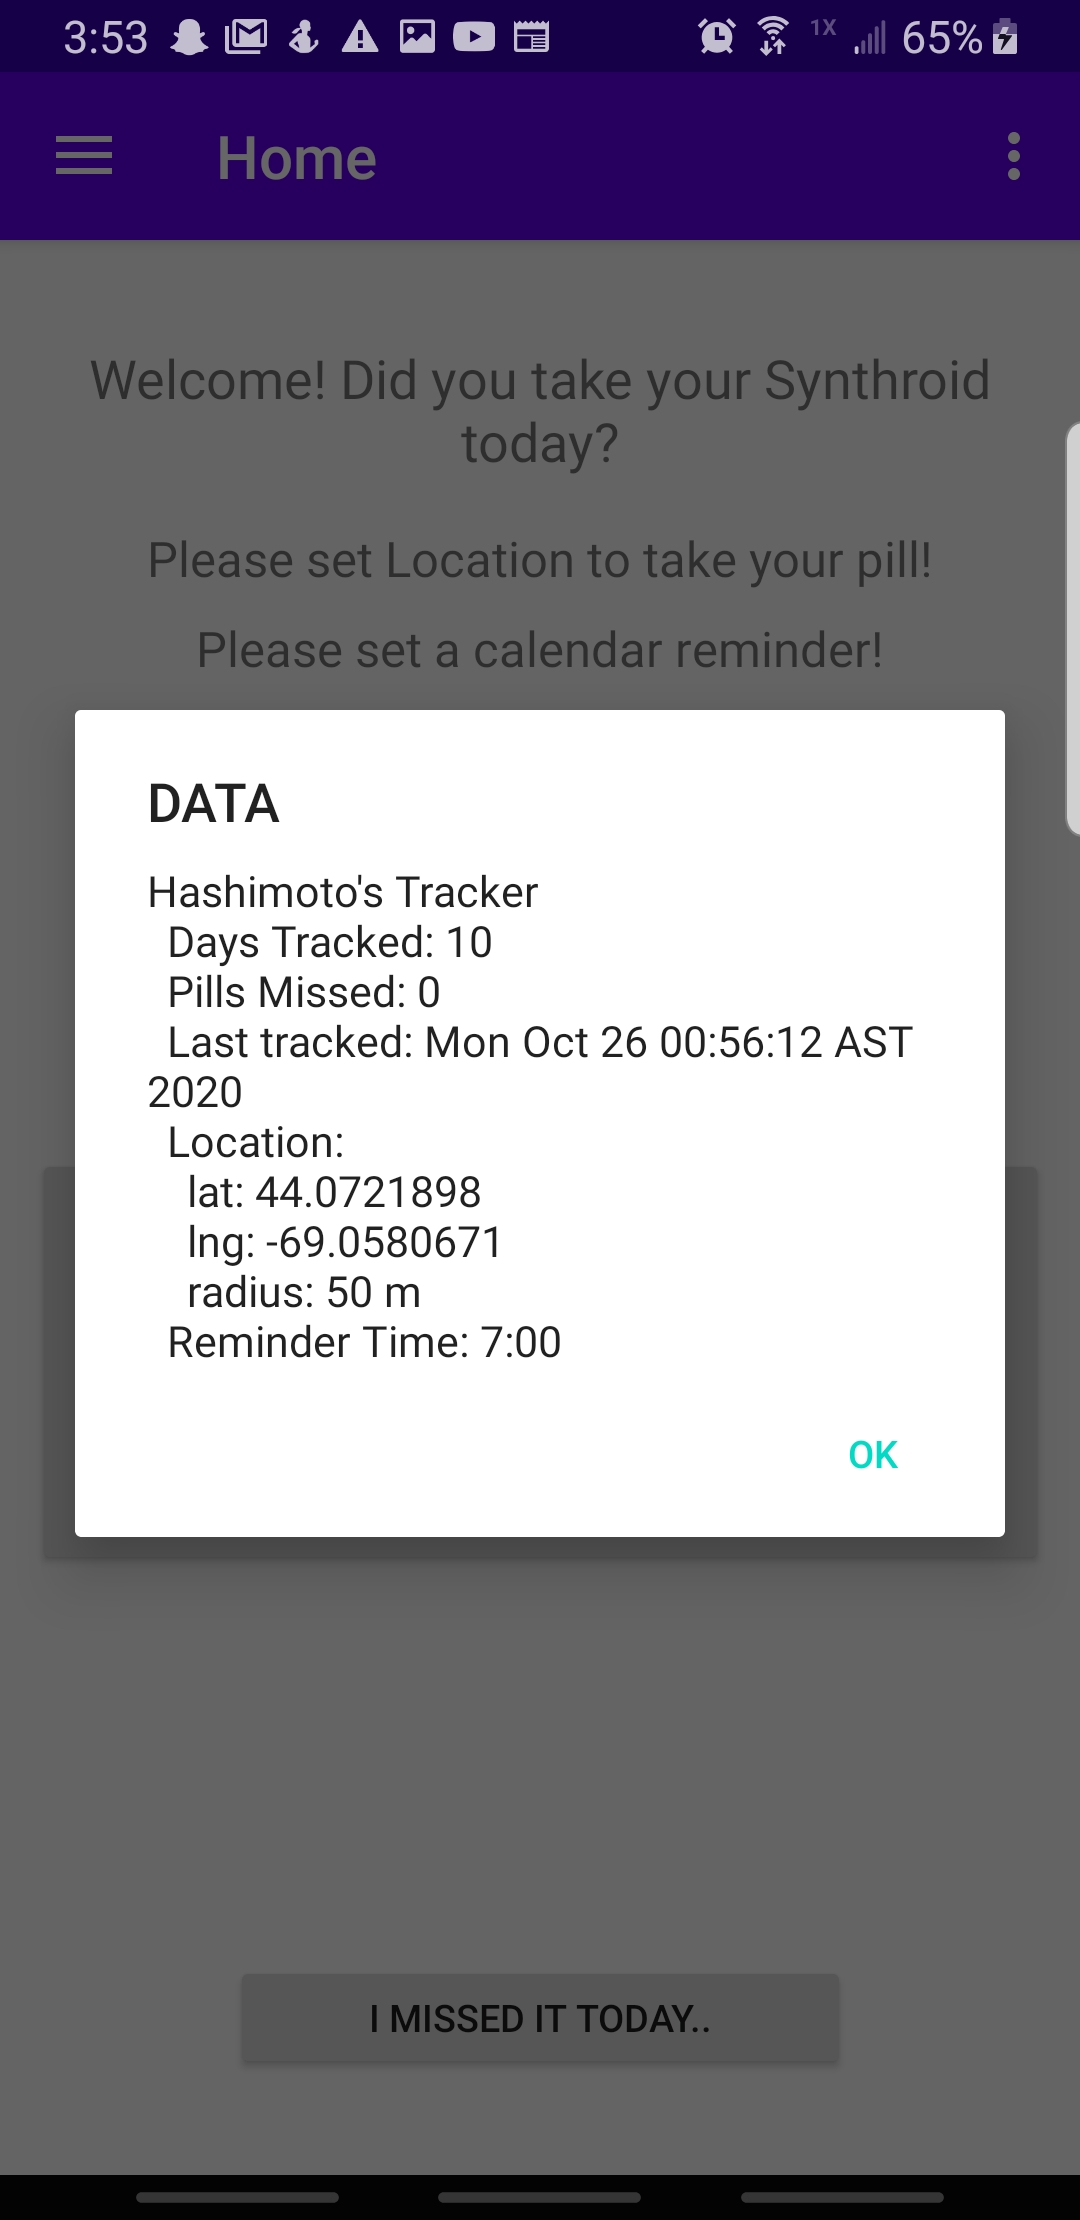
\includegraphics[scale= .1]{img/data.jpg}
\caption{The Database Information}
\label{fig:database} 
\end{figure}

\subsection{Database Information}
On the top right of the application is the Database Information Button. By pressing this button the user will see an up to date instance of all the information in their local database.

\section{Discussion}
This application is a good tool for any person suffering from hypothyroidism and need to improve their medication usage consistency. In the future implementing a cloud based database as well as a local one would allow for more data to be tracked. This application could also be used in a clinical situation to track patients medication consistency between appointments as well.

In designing this application there could be improved code modularity and scalability. In future iteration I hope to implement more robust code Fragment re-usability and User Interface Layout. The Layout that is currently in use is works on well on the screen dimensions of a Samsung Galaxy S8, but has not been tested on other layouts and screen sizes. As an improvement from Lab 2, this application using a ConstraintLayout,and uses a BroadcastReciever as well as multiple Fragments supported by a main Activity. That said, but I would still like to improve my application with more robust threading. 

In the development of this application the Android Developer Studio Documentation website and multiple other sources were invaluable.\citep{AndroidDocs} The PendingIntent and Intent documentation contributed greatly to this effort. \citep{IntentDocs} When working on the database functionality the Room with a view Codelab Tutorial was very helpful.\citep{Room} The Spotify Android SDK as well as the SmartLocation Library were very good resources.\citep{SmartLocation}

\section{Conclusion}
In further iterations of this application, I think a more fluid user interface and the ability to log in the user as well as integrate Amazon AWS rather than simply a local database would be good. As mentioned before the reality of multiple diseases affecting one patient allows for many further improvements to this application. The ability track your medication usage over time is integral to health. This was a very interesting lab and I look forward to the added complexity. 

\bibliographystyle{plain}
\bibliography{references}
\end{document}
